\documentclass[conference]{IEEEtran}
\usepackage{graphicx} % Required for inserting images

\title{TP3 Report - Perception and AI}
\author{\IEEEauthorblockN{Bruno Luiz Dias Alves de Castro}
\IEEEauthorblockA{\textit{ESIEE Paris}}
\and
\IEEEauthorblockN{Victor Gabriel Mendes Sündermann}
\IEEEauthorblockA{\textit{ESIEE Paris}}
}
\date{February 2024}

\begin{document}

\maketitle

\section{Introduction}

Object counting is a process in Computer Vision where, as the name implies, aims to count how many instances of a certain object appear in an image. This process can be used in various areas and can bring about great advantages, such as: resource optimization, improved security, informed decision making, and other.

This can be done in more traditional ways, using state-of-the-art image segmentation methods, such as threshold or watershed, or by more complex and advanced methods like Artificial Intelligence and Neural Networks.

With the decrease in cost of hardware and Artificial Intelligence becoming more widespread, it is necessary to embrace this new technology and find ways use it in common contexts. Jetson Nano is platform designed by NVIDIA that can run multiple parallel neural networks with different applications, this micro computer aims to be the main platform for development of Neural Network applications.
\subsection{Objectives}

The objectives from this practical work are to implement a people counting application that uses both traditional methods and AI, deploy it on the Jetson Nano platform and compare the results between these two methods based on efficiency, execution time and accuracy.

\section{Data preparation}

The data utilized in this work was captured by a depth camera, the images generated are in gray-scale where the brighter a section is the further it is from the camera. Before using it to create the dataset it is necessary to normalize the data, done with the following code in Python.

Now that the images are ready to be used we need to annotate them, apply augmentation and create the dataset, in order to do this we decided to work with the framework \textit{\textbf{Roboflow}}.

\subsection{Roboflow}

\textit{\textbf{Roboflow}} is a web framework focused on data preparation and dataset development. It provides us with all the tools needed for classifying and prepossess our images. It also provides us easy methods of deployment, such as an API, to better import our datasets into our projects without the need to juggle files around.

The dataset prepared with \textit{\textbf{Robolow}} was imported into a \textit{\textbf{Python Notebook}} in order to train the network, afterwards the weights are exported to \textit{\textbf{Jetson Nano}} to test the network in said environment.

\section{Development}

Among all the technologies used during this project, a few can be highlighted:

\begin{itemize}
    \item \textit{\textbf{Ultralytics}}: a library that helps us retrieving data such as performance and specifications from our CPU.
    \item \textit{\textbf{YOLO}}: a real-time object detection system from \textit{\textbf{Ultralytics}}, trained in our project.
    \item \textit{\textbf{OpenCV}}: a optimized Computer Vision library that provides tools and hardware.
    \item \textit{\textbf{Jetson Nano}}: NVIDIA's platform for development of Neural Network Applications.
\end{itemize}

We decided to use YOLO as the detection network because it is a state of the art system, being both fast and accurate when compared to other famous systems, like RetinaNet or SSD.

An essential part in this work is data preparation, in order for the network to be as effective as possible we created a database comprised of 50 annotated images. We applied various augmentation methods in the images to further train our network, resulting in a total of 110 images divided as 82\% training, 9\% validation and 9\% testing.

\subsection{Neural Network Implementation}

The neural network utilized in this project is very similar to that of the previous practical work, we used the model Yolov8, from the Ultralytics library and trained it with 25 epochs. The initial training was done in a Google Colab environment and the final weights were saved and exported to be used in Jetson Nano.

\subsubsection{Colab Results}

After training the network and testing it, we can see that the results were great. The capacity of our network to identify and correctly label people shows that the dataset and epochs were enough for it to learn. 

However we can also observe in Fig. 2 that it is not perfect, when the people approach the center of the image and are closer to each other the network may detect a third person, or detect another a second time.

\begin{figure}[ht!]
    \centering
    \begin{minipage}[b]{0.22\textwidth}
        \centering
        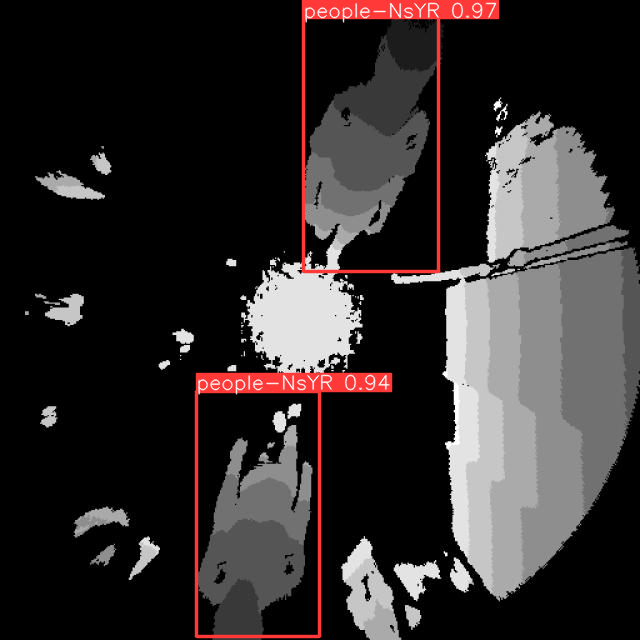
\includegraphics[width=\textwidth]{Images/network/NetRes2.png}
        \caption{Original image}\label{fig:NetRes3}
    \end{minipage}
    \hfill
    \begin{minipage}[b]{0.22\textwidth}
        \centering
        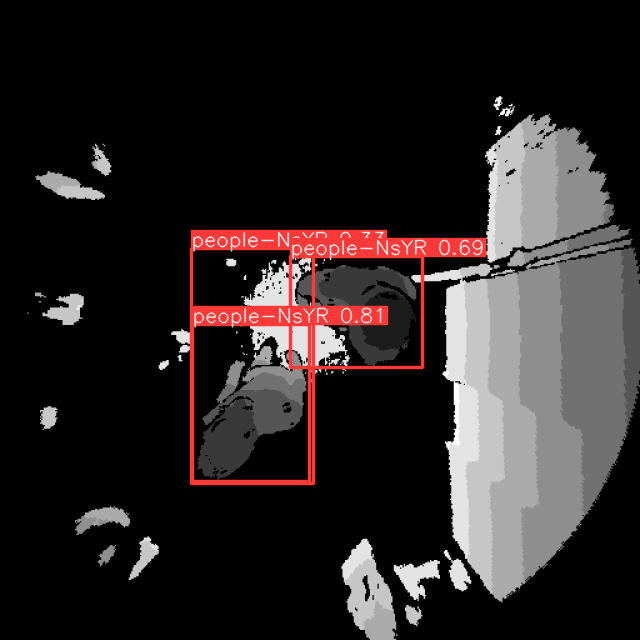
\includegraphics[width=\textwidth]{Images/network/NetRes3.png}
        \caption{Extracted background}\label{fig:NetRes3}
    \end{minipage}
\end{figure}

\subsubsection{Jetson Nano Results}

The connection to the Jetson Nano platform was done through the SSH protocol, we exported only the weights so that we would not need to train the network a second time, and imported pictures to conduct the experiments.

Unfortunately our results within the platform were not promising, in this case the results were terrible and the network was detecting multiple people on various places over the image. The group could not record the results during the demo class, and did not manage to connect to the platform on the following week to reproduce the results, therefore we do not have pictures to describe this part of the experiment.

\subsection{A Classical Implementation}

Machine Learning algorithms, though powerful, are no silver bullet. Depending on the scale of our problem, and the expected accuracy and results, a neural networks may just be overkill.

Looking back at our problem, we have a well controlled environment, with a fixed camera and a simple task counting people. This suggest that, maybe a classical algorithm deliver results close to the one we got with the neural network, while using less resources and running faster.

We decided to implement some simple image processing techniques to reach the same results. The approach is as follows:

\begin{itemize}
    \item Extract the background from the scene, and use it as "ground truth";
    \item Subtract our background from the image we want to process;
    \item Apply some image topology algorithms (such as opening and closing) to remove noise and refine the results;
    \item Count the "blobs" we have in the image and label the people we found in it;
\end{itemize}

\subsubsection{Background}

Processing the background is an easy test. Knowing the camera stays fixed, and the elements in the scenery do not change, it is just a matter of selecting an image with no people on them, or removing the people in one of them, assuming the are not over any background elements.

For our implementation, the image selected, and its extracted background, are below. On top of the people extracting (that in this case, was done by manually setting the rectangle containing them to zero), we also applied one image processing technique on top, a closing, using a 7x7 kernel, to remove noise and perform a better background extraction.

\begin{figure}[ht!]
    \centering
    \begin{minipage}[b]{0.22\textwidth}
        \centering
        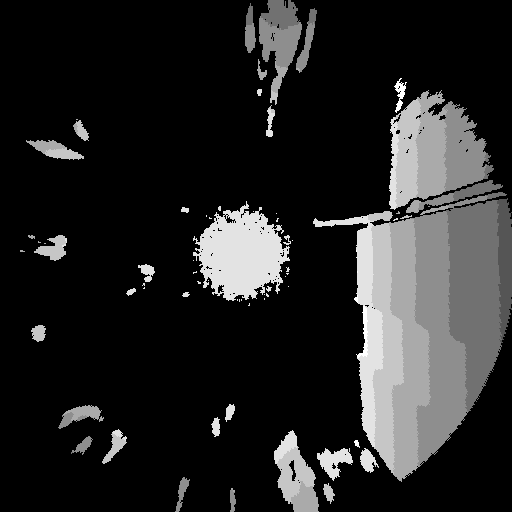
\includegraphics[width=\textwidth]{Images/classical/112.png}
        \caption{Original image}\label{fig:NetRes3}
    \end{minipage}
    \hfill
    \begin{minipage}[b]{0.22\textwidth}
        \centering
        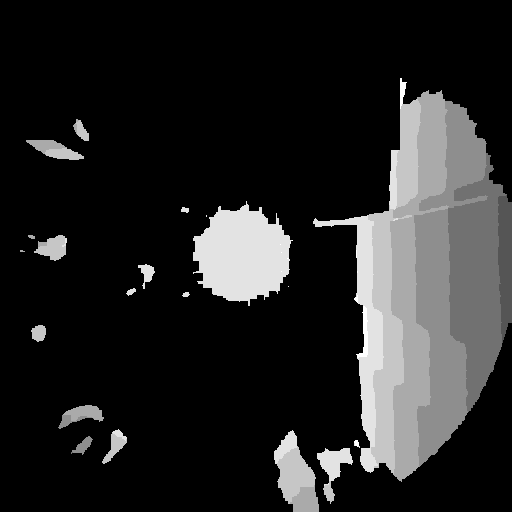
\includegraphics[width=\textwidth]{Images/classical/backgroung.png}
        \caption{Extracted background}\label{fig:NetRes3}
    \end{minipage}
\end{figure}

\subsubsection{Background removal}

During this part, we extract the background we just processed, from the image we wish to process. This removal already give us great results, and almost the entirety of the background is removed. Bellow, we have the same image before and after the background removed. Along with the extraction, we performed an erosion, and a closing in the image, to further isolate the people in it.

\begin{figure}[ht!]
    \centering
    \begin{minipage}[b]{0.22\textwidth}
        \centering
        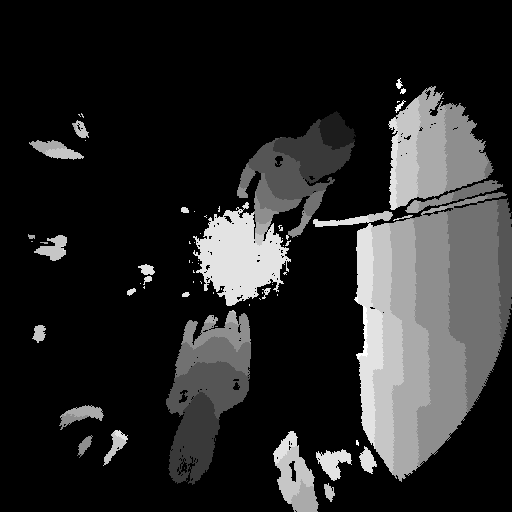
\includegraphics[width=\textwidth]{Images/classical/163.png}
        \caption{Original image}\label{fig:NetRes3}
    \end{minipage}
    \hfill
    \begin{minipage}[b]{0.22\textwidth}
        \centering
        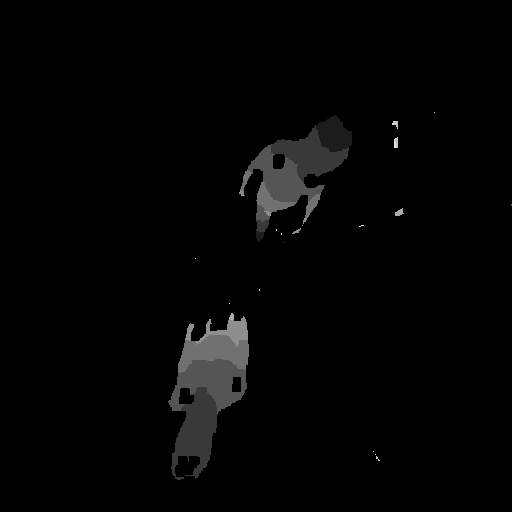
\includegraphics[width=\textwidth]{Images/classical/163-no-back.png}
        \caption{Extracted background}\label{fig:NetRes3}
    \end{minipage}
\end{figure}

\subsubsection{People detecting}

After the background removal, we just extracted the contours in the image, and after setting  the upper and lower bounds, we traced the "blobs" we had in the image. The result is available in the following image.

\begin{figure}[ht!]
    \centering
    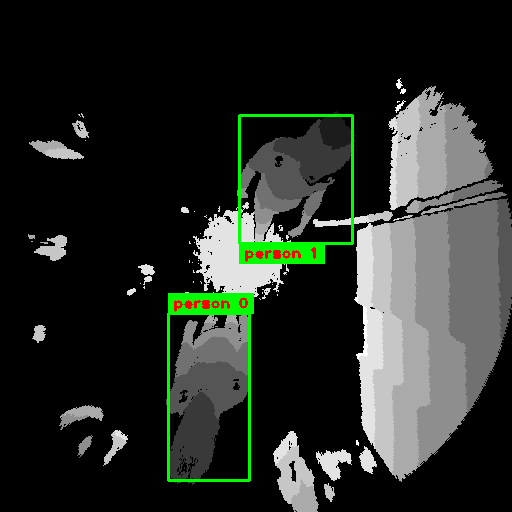
\includegraphics[width=0.4\textwidth]{Images/classical/163-result.png}
    \caption{Result}\label{fig:ir-results}
\end{figure}

\subsubsection{Drawbacks}

Even though we were able to achieve results closer to the neural network with this approach, it does have its drawbacks.

The most obvious one, it that a given background will only work with a fixed camera, in the same scenery. If the camera moves or the background changes, this approach will fail, and a new background must be processed. There are ways to automate this background detection though, but as the problem gets more complex, less viable the classical algorithms prove to be.

One other big issue with this alternative, is that even though it does perform well with this problem, we could as well say that it count "whatever" moves in the scenery, not only people. The algorithm is only really capable of extracting objects from the background, and do not differentiate at all between this objects. If, lets say, a dog, passes in the video footage, it may as well be recognized as a person.

Though our approach perform well, it only does because the environment is well controlled and the variables do not change. In other applications, such as autonomous cars, these classical algorithms may start to fail a lot, and that is when we should start thinking about implementing more robust solutions, such as neural networks. But if we are working on a simple problem, with no big consequences for failing, maybe the speed and simplicity of a classical algorithm proves to be enough.

\section{Conclusion}

In our local implementation of the network the results were satisfying, however with Jetson Nano the accuracy of our network plummeted, we do not know the reason for this decrease and should look into this further, however we managed to see the potential of the Jetson Platform on the development of AI applications, with its compact size and high computational power.

When comparing the two approaches we observe that the classical has the upper hand, the results were better and because it relies on mathematical and morphological operations it requires less time and computing power, but once again, this scenario has a static camera, therefore the results in a new environment may vary, as the background will need to be determined once more.

Overall this project was essential to deepen our knowledge on Artificial Intelligence and Image Segmentation, the chance to work with a high-end platform like Jetson Nano is also greatly appreciated, it is unfortunate that the results were not promising, however with more time, data, resources and further experiments we are sure to achieve great results and utilize Jetson to it's full potential.

\end{document}